\documentclass[tikz,border=3pt]{standalone}
\usepackage[utf8]{inputenc}
\usepackage[T1]{fontenc}
\usepackage{lmodern}
\renewcommand{\familydefault}{\sfdefault}
\usepackage{sansmath}\sansmath
\usepackage{chemfig}
\usepackage{pgfplots}\pgfplotsset{compat=1.18,/pgf/number format/use comma,/pgf/number format/1000 sep={.}}
\usetikzlibrary{arrows.meta,calc,positioning,decorations.pathmorphing,patterns}
% paleta del sitio
\definecolor{nar}{HTML}{E8680C}\definecolor{narc}{HTML}{FFB35C}\definecolor{hielo}{HTML}{FFF3E8}
\definecolor{tinta}{HTML}{1D1D1F}\definecolor{gris}{HTML}{6E6E73}\definecolor{lila}{HTML}{7C5CF0}
\definecolor{azul}{HTML}{2F6FD6}\definecolor{menta}{HTML}{17A673}\definecolor{coral}{HTML}{E8342A}
\tikzset{cel/.style={draw=gris,fill=hielo,line width=0.9pt},nuc/.style={draw=gris!70,line width=0.6pt},
fib/.style={gris!55,line width=0.35pt},eti/.style={font=\footnotesize,text=tinta,align=center},
num/.style={circle,draw=nar,fill=white,text=nar,font=\small\bfseries,inner sep=1.2pt,minimum size=13pt},
fl/.style={-{Stealth[length=2.6mm]},gris,line width=0.9pt}}
\begin{document}
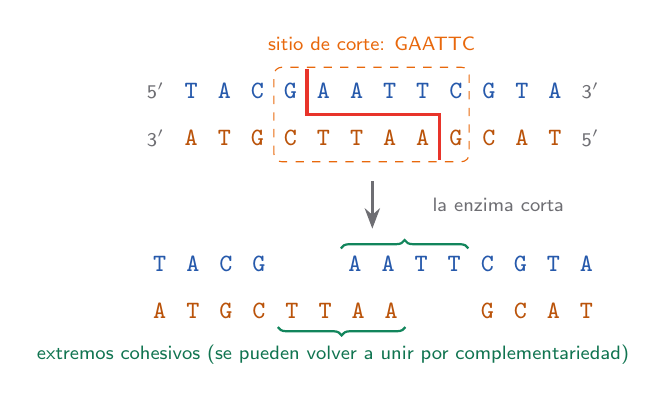
\begin{tikzpicture}[font=\small]
\node[font=\ttfamily\small,text=azul!80!black] at (0,0.3) {T};
\node[font=\ttfamily\small,text=azul!80!black] at (0.42,0.3) {A};
\node[font=\ttfamily\small,text=azul!80!black] at (0.84,0.3) {C};
\node[font=\ttfamily\small,text=azul!80!black] at (1.26,0.3) {G};
\node[font=\ttfamily\small,text=azul!80!black] at (1.68,0.3) {A};
\node[font=\ttfamily\small,text=azul!80!black] at (2.1,0.3) {A};
\node[font=\ttfamily\small,text=azul!80!black] at (2.52,0.3) {T};
\node[font=\ttfamily\small,text=azul!80!black] at (2.94,0.3) {T};
\node[font=\ttfamily\small,text=azul!80!black] at (3.36,0.3) {C};
\node[font=\ttfamily\small,text=azul!80!black] at (3.78,0.3) {G};
\node[font=\ttfamily\small,text=azul!80!black] at (4.2,0.3) {T};
\node[font=\ttfamily\small,text=azul!80!black] at (4.62,0.3) {A};
\node[font=\ttfamily\small,text=nar!80!black] at (0,-0.3) {A};
\node[font=\ttfamily\small,text=nar!80!black] at (0.42,-0.3) {T};
\node[font=\ttfamily\small,text=nar!80!black] at (0.84,-0.3) {G};
\node[font=\ttfamily\small,text=nar!80!black] at (1.26,-0.3) {C};
\node[font=\ttfamily\small,text=nar!80!black] at (1.68,-0.3) {T};
\node[font=\ttfamily\small,text=nar!80!black] at (2.1,-0.3) {T};
\node[font=\ttfamily\small,text=nar!80!black] at (2.52,-0.3) {A};
\node[font=\ttfamily\small,text=nar!80!black] at (2.94,-0.3) {A};
\node[font=\ttfamily\small,text=nar!80!black] at (3.36,-0.3) {G};
\node[font=\ttfamily\small,text=nar!80!black] at (3.78,-0.3) {C};
\node[font=\ttfamily\small,text=nar!80!black] at (4.2,-0.3) {A};
\node[font=\ttfamily\small,text=nar!80!black] at (4.62,-0.3) {T};
\draw[nar,dashed,rounded corners=1mm] (1.05,-0.6) rectangle (3.53,0.6);
\node[eti,font=\scriptsize,text=nar] at (2.29,0.9) {sitio de corte: GAATTC};
\draw[coral,very thick] (1.47,0.58)--(1.47,0)--(3.15,0)--(3.15,-0.58);
\node[font=\scriptsize,text=gris] at (-0.45,0.3) {5$^\prime$};\node[font=\scriptsize,text=gris] at (5.07,0.3) {3$^\prime$};
\node[font=\scriptsize,text=gris] at (-0.45,-0.3) {3$^\prime$};\node[font=\scriptsize,text=gris] at (5.07,-0.3) {5$^\prime$};
\draw[fl] (2.3,-0.85)--(2.3,-1.45);\node[eti,font=\scriptsize,text=gris] at (3.9,-1.15) {la enzima corta};
\node[font=\ttfamily\small,text=azul!80!black] at (-0.4,-1.9) {T};
\node[font=\ttfamily\small,text=azul!80!black] at (0.02,-1.9) {A};
\node[font=\ttfamily\small,text=azul!80!black] at (0.44,-1.9) {C};
\node[font=\ttfamily\small,text=azul!80!black] at (0.86,-1.9) {G};
\node[font=\ttfamily\small,text=nar!80!black] at (-0.4,-2.5) {A};
\node[font=\ttfamily\small,text=nar!80!black] at (0.02,-2.5) {T};
\node[font=\ttfamily\small,text=nar!80!black] at (0.44,-2.5) {G};
\node[font=\ttfamily\small,text=nar!80!black] at (0.86,-2.5) {C};
\node[font=\ttfamily\small,text=nar!80!black] at (1.28,-2.5) {T};
\node[font=\ttfamily\small,text=nar!80!black] at (1.7,-2.5) {T};
\node[font=\ttfamily\small,text=nar!80!black] at (2.12,-2.5) {A};
\node[font=\ttfamily\small,text=nar!80!black] at (2.54,-2.5) {A};
\node[font=\ttfamily\small,text=azul!80!black] at (2.08,-1.9) {A};
\node[font=\ttfamily\small,text=azul!80!black] at (2.5,-1.9) {A};
\node[font=\ttfamily\small,text=azul!80!black] at (2.92,-1.9) {T};
\node[font=\ttfamily\small,text=azul!80!black] at (3.34,-1.9) {T};
\node[font=\ttfamily\small,text=azul!80!black] at (3.76,-1.9) {C};
\node[font=\ttfamily\small,text=azul!80!black] at (4.18,-1.9) {G};
\node[font=\ttfamily\small,text=azul!80!black] at (4.6,-1.9) {T};
\node[font=\ttfamily\small,text=azul!80!black] at (5.02,-1.9) {A};
\node[font=\ttfamily\small,text=nar!80!black] at (3.76,-2.5) {G};
\node[font=\ttfamily\small,text=nar!80!black] at (4.18,-2.5) {C};
\node[font=\ttfamily\small,text=nar!80!black] at (4.6,-2.5) {A};
\node[font=\ttfamily\small,text=nar!80!black] at (5.02,-2.5) {T};
\draw[menta!80!black,thick,decorate,decoration={brace,mirror,amplitude=3pt}] (1.1,-2.7)--(2.72,-2.7);
\draw[menta!80!black,thick,decorate,decoration={brace,amplitude=3pt}] (1.9,-1.7)--(3.52,-1.7);
\node[eti,font=\scriptsize,text=menta!70!black] at (1.8,-3.05) {extremos cohesivos (se pueden volver a unir por complementariedad)};
\end{tikzpicture}
\end{document}
